\documentclass[10pt,]{article}
\usepackage{lmodern}
\usepackage{amssymb,amsmath}
\usepackage{ifxetex,ifluatex}
\usepackage{fixltx2e} % provides \textsubscript
\ifnum 0\ifxetex 1\fi\ifluatex 1\fi=0 % if pdftex
  \usepackage[T1]{fontenc}
  \usepackage[utf8]{inputenc}
\else % if luatex or xelatex
  \ifxetex
    \usepackage{mathspec}
    \usepackage{xltxtra,xunicode}
  \else
    \usepackage{fontspec}
  \fi
  \defaultfontfeatures{Mapping=tex-text,Scale=MatchLowercase}
  \newcommand{\euro}{€}
\fi
% use upquote if available, for straight quotes in verbatim environments
\IfFileExists{upquote.sty}{\usepackage{upquote}}{}
% use microtype if available
\IfFileExists{microtype.sty}{%
\usepackage{microtype}
\UseMicrotypeSet[protrusion]{basicmath} % disable protrusion for tt fonts
}{}
\usepackage[margin=1in]{geometry}
\usepackage{color}
\usepackage{fancyvrb}
\newcommand{\VerbBar}{|}
\newcommand{\VERB}{\Verb[commandchars=\\\{\}]}
\DefineVerbatimEnvironment{Highlighting}{Verbatim}{commandchars=\\\{\}}
% Add ',fontsize=\small' for more characters per line
\usepackage{framed}
\definecolor{shadecolor}{RGB}{248,248,248}
\newenvironment{Shaded}{\begin{snugshade}}{\end{snugshade}}
\newcommand{\KeywordTok}[1]{\textcolor[rgb]{0.13,0.29,0.53}{\textbf{{#1}}}}
\newcommand{\DataTypeTok}[1]{\textcolor[rgb]{0.13,0.29,0.53}{{#1}}}
\newcommand{\DecValTok}[1]{\textcolor[rgb]{0.00,0.00,0.81}{{#1}}}
\newcommand{\BaseNTok}[1]{\textcolor[rgb]{0.00,0.00,0.81}{{#1}}}
\newcommand{\FloatTok}[1]{\textcolor[rgb]{0.00,0.00,0.81}{{#1}}}
\newcommand{\CharTok}[1]{\textcolor[rgb]{0.31,0.60,0.02}{{#1}}}
\newcommand{\StringTok}[1]{\textcolor[rgb]{0.31,0.60,0.02}{{#1}}}
\newcommand{\CommentTok}[1]{\textcolor[rgb]{0.56,0.35,0.01}{\textit{{#1}}}}
\newcommand{\OtherTok}[1]{\textcolor[rgb]{0.56,0.35,0.01}{{#1}}}
\newcommand{\AlertTok}[1]{\textcolor[rgb]{0.94,0.16,0.16}{{#1}}}
\newcommand{\FunctionTok}[1]{\textcolor[rgb]{0.00,0.00,0.00}{{#1}}}
\newcommand{\RegionMarkerTok}[1]{{#1}}
\newcommand{\ErrorTok}[1]{\textbf{{#1}}}
\newcommand{\NormalTok}[1]{{#1}}
\usepackage{graphicx}
\makeatletter
\def\maxwidth{\ifdim\Gin@nat@width>\linewidth\linewidth\else\Gin@nat@width\fi}
\def\maxheight{\ifdim\Gin@nat@height>\textheight\textheight\else\Gin@nat@height\fi}
\makeatother
% Scale images if necessary, so that they will not overflow the page
% margins by default, and it is still possible to overwrite the defaults
% using explicit options in \includegraphics[width, height, ...]{}
\setkeys{Gin}{width=\maxwidth,height=\maxheight,keepaspectratio}
\ifxetex
  \usepackage[setpagesize=false, % page size defined by xetex
              unicode=false, % unicode breaks when used with xetex
              xetex]{hyperref}
\else
  \usepackage[unicode=true]{hyperref}
\fi
\hypersetup{breaklinks=true,
            bookmarks=true,
            pdfauthor={Carlo Michaelis, 573479; Lukas Ruff, 572521},
            pdftitle={Projektaufgaben Block 1},
            colorlinks=true,
            citecolor=blue,
            urlcolor=blue,
            linkcolor=magenta,
            pdfborder={0 0 0}}
\urlstyle{same}  % don't use monospace font for urls
\setlength{\parindent}{0pt}
\setlength{\parskip}{6pt plus 2pt minus 1pt}
\setlength{\emergencystretch}{3em}  % prevent overfull lines
\setcounter{secnumdepth}{5}

%%% Use protect on footnotes to avoid problems with footnotes in titles
\let\rmarkdownfootnote\footnote%
\def\footnote{\protect\rmarkdownfootnote}

%%% Change title format to be more compact
\usepackage{titling}

% Create subtitle command for use in maketitle
\newcommand{\subtitle}[1]{
  \posttitle{
    \begin{center}\large#1\end{center}
    }
}

\setlength{\droptitle}{-2em}
  \title{Projektaufgaben Block 1}
  \pretitle{\vspace{\droptitle}\centering\huge}
  \posttitle{\par}
  \author{Carlo Michaelis, 573479; Lukas Ruff, 572521}
  \preauthor{\centering\large\emph}
  \postauthor{\par}
  \predate{\centering\large\emph}
  \postdate{\par}
  \date{15 November 2016}

\usepackage{amsthm}
\usepackage{MnSymbol}
\usepackage{theoremref}
\newtheorem{satz}{Satz}
\usepackage{amssymb}
\usepackage{bbm}


\begin{document}

\maketitle


\section{Infinite-Monkey-Theorem}\label{infinite-monkey-theorem}

\subsection{Formulierung und Beweis des
Infinite-Monkey-Theorems}\label{formulierung-und-beweis-des-infinite-monkey-theorems}

Laut dem Infinite-Monkey-Theorem wird ein Affe, der unendlich lange
zufällig auf einer Schreibmaschine tippt, fast sicher jede beliebige
Zeichenkette unendlich oft schreiben. Diese bildhafte Interpretation des
mathematischen Satzes soll der gedanklichen Einordnung von Unendlichkeit
dienen. Das Infinite-Monkey-Theorem ist ein Beispiel für die Anwendung
des Lemmas von Borel-Cantelli. \newline

\begin{satz}[Lemma von Borel-Cantelli] 
Sei $(\Omega, \mathcal{F}, P)$ ein Wahrscheinlichkeitsraum.

a) Ist $(A_n)_{n \in \mathbb{N}}$ eine Folge von Ereignissen mit $\sum_{n \in \mathbb{N}} P(A_n) < \infty$, so gilt 
$$ 
P \left( \limsup_{n \to \infty} A_n \right) = 0.
$$

b) Ist $(A_n)_{n \in \mathbb{N}}$ eine Folge von unabhängigen Ereignissen mit $\sum_{n \in \mathbb{N}} P(A_n) = + \infty$, so gilt 
$$
P \left( \limsup_{n \to \infty} A_n \right) = 1.
$$
\end{satz}

Um das Infinite-Monkey-Theorem formulieren zu können, modellieren wir
zunächst einen geeigneten Wahrscheinlichkeitsraum. Definiere dazu ein
endliches Alphabet \(\Omega := \{\text{a, b, c, } \ldots \}\),
d.h.~\(\Omega\) ist eine Menge von Zeichen (Buchstaben, Satzzeichen,
Zahlen, etc.) mit \(\vert \Omega \vert = n\) für ein
\(n \in \mathbb{N}\). Setze weiter die zugehörige \(\sigma\)-Algebra als
Potenzmenge \(\mathcal{F} := \mathcal{P}(\Omega)\) und definiere das
Wahrscheinlichkeitsmaß \(P\) als diskrete Gleichverteilung,
d.h.~\(P(A) = \frac{\vert A \vert}{\vert \Omega \vert} = \frac{\vert A \vert}{n}\)
für \(A \in \mathcal{F}\). Somit modelliert \((\Omega, \mathcal{F}, P)\)
das Ziehen von Zeichen aus einem Alphabet mit gleicher
Wahtscheinlichkeit. Den Übergang zu Zeichenketten (Folgen von Zeichen
aus dem Alphabet \(\Omega\)) können wir nun mittels des (stets
existierenden und eindeutigen) Produktraumes
\((\Omega^{\mathbb{N}}, \mathcal{F}^{\mathbb{N}}, \mathbb{P})\) mit
\(\mathbb{P} := P^{\mathbb{N}}\) bewerkstelligen. Hiermit können wir das
Infinite-Monkey-Theorem wie folgt formulieren und beweisen: \newline

\begin{satz}[Infinite-Monkey-Theorem]
Betrachte den oben definierten Produktraum $(\Omega^{\mathbb{N}}, \mathcal{F}^{\mathbb{N}}, \mathbb{P})$ von (unendlich langen) Zeichenketten und sei $s = (s_1, \ldots, s_m)^\top \in \Omega^m$ eine beliebige Zeichenkette der Länge $m \in \mathbb{N}$ (String). Definiere zu $k \in \mathbb{N}$ das Ereignis
$$ 
A_{k} := \left\{ \omega = (\omega_j)_{j \in \mathbb{N}} \in \Omega^{\mathbb{N}} \, : \, \omega_k = s_1, \ldots, \omega_{k+m-1} = s_m \right\},
$$
d.h.\ $A_k$ ist das Ereignis, dass String $s$ der Länge $m$ an der Stelle $k$ in einer Zeichenkette beginnt. Dann ist $(A_{jm+1})_{j \in \mathbb{N}_0}$ eine Folge unabhängiger Ereignisse und es gilt
$$
\mathbb{P} \left( \limsup_{j \to \infty} A_{jm+1} \right) = 1.
$$
\end{satz}

\begin{proof}[Beweis]
Es sei $\pi_i: \Omega^{\mathbb{N}} \to \Omega, (\omega_j)_{j \in \mathbb{N}} \mapsto \omega_i$ die $i$-te Koordinatenprojektion auf dem kartesischen Produkt $\Omega^{\mathbb{N}}$. Weiter sei $(I_j)_{j \in \mathbb{N}_0}$ eine Zerlegung von $\mathbb{N}$ in disjunkte Blöcke der Länge $m$, d.h.\ 
$$
\mathbb{N} = \bigcupdot_{j \in \mathbb{N}_0} I_j \qquad \text{mit} \qquad I_j := \bigcup_{k = 1}^m \{jm+k\}, \, j \in \mathbb{N}_0.
$$
Dann folgt für $j \in \mathbb{N}_0$
$$
\begin{aligned}
\mathbb{P}(A_{jm+1}) &= \mathbb{P}\left( \left\{ \omega \, : \, \omega_{jm+1} = s_1, \ldots, \omega_{(j+1)m} = s_m \right\} \right) \\
&= \mathbb{P}\left( \bigcap_{k = 1}^m \pi_{jm+k}^{-1}(\{s_k\}) \right) \\
&= \prod_{k=1}^m P(\{s_k\}) = \left(\frac{1}{n} \right)^m,
\end{aligned}
$$
da $\mathbb{P} = P^{\mathbb{N}}$ Produktmaß ist. Weiter folgt für $j_1, j_2 \in \mathbb{N}_0, j_1 \not = j_2$:
$$
\begin{aligned}
\mathbb{P} \left( A_{j_1m+1} \cap A_{j_2m+1} \right) &= \mathbb{P}\left( \left\{ \omega \, : \, \omega_{j_1m+1} = s_1, \ldots, \omega_{(j_1+1)m} = s_m \right\} \cap \left\{ \omega \, : \, \omega_{j_2m+1} = s_1, \ldots, \omega_{(j_2+1)m} = s_m \right\} \right) \\
&= \mathbb{P}\left( \left( \bigcap_{k = 1}^m \pi_{j_1m+k}^{-1}(\{s_k\}) \right) \cap \left( \bigcap_{k = 1}^m \pi_{j_2m+k}^{-1}(\{s_k\}) \right) \right) \\
&= \left( \prod_{k=1}^m P(\{s_k\}) \right)^2 = \left(\frac{1}{n} \right)^m  \left(\frac{1}{n} \right)^m = \mathbb{P}(A_{j_1m+1}) \cdot \mathbb{P}(A_{j_2m+1}),
\end{aligned}
$$
da $I_{j_1} \cap I_{j_2} = \emptyset$ für $j_1 \not= j_2$. Somit ist $(A_{jm+1})_{j \in \mathbb{N}_0}$ eine Folge unabhängiger Ereignisse mit
$$
\sum_{j \in \mathbb{N}_0} P(A_{jm+1}) = \sum_{j \in \mathbb{N}_0} \left(\frac{1}{n}\right)^m = + \infty.
$$
D.h.\ mit Teil b) des Lemma von Borel-Cantelli folgt die Behauptung.
\end{proof}

Es gilt also

\[
\begin{aligned}
\mathbb{P} \left( \limsup_{j \to \infty} A_{jm+1} \right) &= \mathbb{P} \left( \bigcap_{j \in \mathbb{N}_0} \bigcup_{k \geq j} A_{km+1} \right) \\
&= \mathbb{P} \left( \left\{ \omega \in \Omega^{\mathbb{N}}  \, : \, \forall j \in \mathbb{N}_0 \, \exists k \geq j : \omega \in A_{km+1} \right\} \right) \\
&= \mathbb{P} \left( \left\{ \omega \in \Omega^{\mathbb{N}}  \, : \, \omega \in A_{jm+1} \text{ für unendlich viele } j \in \mathbb{N}_0 \right\} \right) = 1,
\end{aligned}
\] d.h.~jeder beliebige String \(s\) der Länge \(m\) erscheint fast
sicher unendlich oft.

\subsection{Simulation eines Infinite-Monkey
Experiments}\label{simulation-eines-infinite-monkey-experiments}

In diesem Abschnitt wollen wir das Infinite-Monkey-Theorem experimentell
simulieren. Wir schreiben hierzu eine R-Funktion die solange zufällig
Zeichen aus dem Alphabet \(\Omega = \{a, b, \ldots, y, z\}\) mit
gleicher Wahrscheinlichkeit (d.h.~\(\frac{1}{26}\)) auswählt, bis eine
vorgegebene Zeichenkette
\(s = (s_1, \ldots, s_m)^\top \in \Omega^m, m \in \mathbb{N},\)
vollständig erschienen ist. Die R-Funktion gibt dann die Anzahl der bis
zum Erscheinen der Zeichenkette \(s\) gezogenen Zeichen zurück. Damit
simulieren wir die Zufallsvariable
\(X: \Omega^{\mathbb{N}} \to \mathbb{N}\) mit \[ 
X(\omega) = \min\{k+m-1 \, : \, \omega_k = s_1, \ldots, \omega_{k+m-1} = s_m \text{ für } k \in \mathbb{N} \}
\]

Wir haben die Funktion wie folgt in R implementiert:\footnote{Eine
  effizientere Implementierung wäre je Schleifendurchlauf eine größere
  Anzahl an Zeichen zu generieren und den resultierenden Zeichen-Block
  mit einem Fenster nach \texttt{strTarget} zu durchsuchen. Dabei muss
  beachtet werden, dass \texttt{strTarget} auch in der Überlappung
  zweier Blöcke erscheinen könnte. Für unsere Untersuchung ist eine
  vereinfachte (ineffiziente) Implementierung jedoch ausreichend. Für
  große Samples oder einen langen String \texttt{strTarget} sollte
  jedoch auf jeden Fall eine effizientere Implementierung herangezogen
  werden.}

\newpage

\begin{Shaded}
\begin{Highlighting}[]
\NormalTok{fnInfiniteMonkey <-}\StringTok{ }\NormalTok{function(strTarget) \{}
  \CommentTok{# This function is a simulation of the Infinite-Monkey-Theorem. It generates a}
  \CommentTok{# random sequence of letters until a given target string appears.}
  \CommentTok{# }
  \CommentTok{# Args:}
  \CommentTok{#   strTarget: The target string which should be matched}
  \CommentTok{#   }
  \CommentTok{# Returns:}
  \CommentTok{#   The number of generated letters until the target string appeared}
  
  \CommentTok{# Split target string to vector of chars}
  \NormalTok{vecCharTarget <-}\StringTok{ }\KeywordTok{strsplit}\NormalTok{(strTarget, }\StringTok{""}\NormalTok{)[[}\DecValTok{1}\NormalTok{]]}
  \CommentTok{# Get the number of letters in target string}
  \NormalTok{nTarget <-}\StringTok{ }\KeywordTok{length}\NormalTok{(vecCharTarget)}
  
  \CommentTok{# Set counting variable (at least nTarget letters needed)}
  \NormalTok{nCounter <-}\StringTok{ }\NormalTok{nTarget}
  
  \CommentTok{# Switch on the monkey (i.e. sample the first nTarget letters)}
  \NormalTok{vecLetterSeqTail <-}\StringTok{ }\KeywordTok{sample}\NormalTok{(letters, nTarget, }\DataTypeTok{replace =} \OtherTok{TRUE}\NormalTok{)}
  
  \CommentTok{# Let the monkey type until target string was written}
  \NormalTok{while(!}\KeywordTok{identical}\NormalTok{(vecCharTarget, vecLetterSeqTail)) \{}
    
    \CommentTok{# Let the monkey hit another key (sample next letter) and store in }
    \CommentTok{# vecLetterSeqTail (first in, first out)}
    \NormalTok{if (nTarget ==}\StringTok{ }\DecValTok{1}\NormalTok{) \{}
      \NormalTok{vecLetterSeqTail <-}\StringTok{ }\KeywordTok{sample}\NormalTok{(letters, }\DecValTok{1}\NormalTok{)}
    \NormalTok{\} else \{}
      \NormalTok{vecLetterSeqTail <-}\StringTok{ }\KeywordTok{c}\NormalTok{(vecLetterSeqTail[}\DecValTok{2}\NormalTok{:nTarget], }
                            \KeywordTok{sample}\NormalTok{(letters, }\DecValTok{1}\NormalTok{, }\DataTypeTok{replace =} \OtherTok{TRUE}\NormalTok{))}
    \NormalTok{\}}
    \CommentTok{# Count}
    \NormalTok{nCounter <-}\StringTok{ }\NormalTok{nCounter +}\StringTok{ }\DecValTok{1}
  \NormalTok{\}}
  
  \CommentTok{# Return the length of the generated letter sequence}
  \KeywordTok{return}\NormalTok{(nCounter)}
\NormalTok{\}}
\end{Highlighting}
\end{Shaded}

\begin{figure}[htbp]
\centering
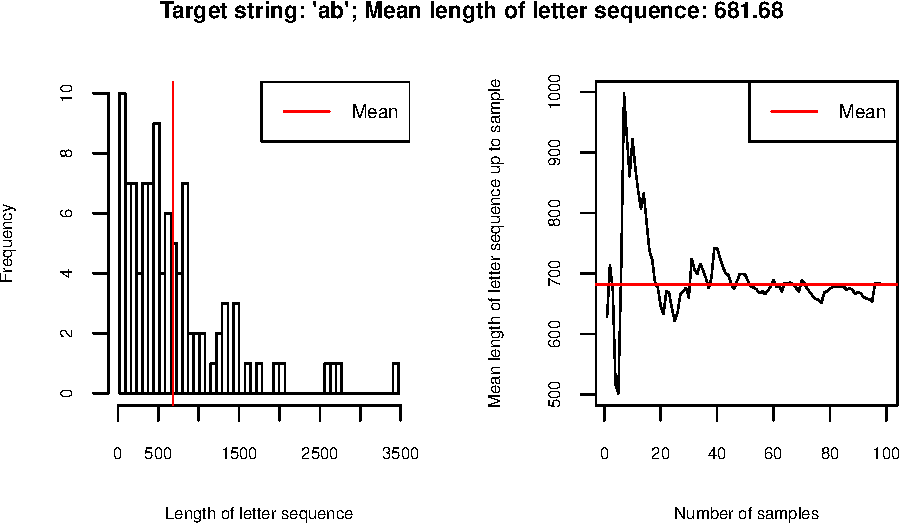
\includegraphics{project1_files/figure-latex/Infinite-Monkey Simulation-1.pdf}
\caption{Histogram of letter sequence lengths and mean letter sequence
length by number of samples.\label{fig:plotMonkey}}
\end{figure}

In Figure \ref{fig:plotMonkey} haben wir ein Histogramm der simulierten
Anzahlen von Zeichen und die durchschnittliche Anzahl von Zeichen, bis
die Zeichenkette \texttt{\textquotesingle{}ab\textquotesingle{}}
vollständig erschienen ist, für \(10^4\) Samples geplottet. Wir können
sehen, dass die Anzahl von Zeichen \(X\) einer rechtsschiefen Verteilung
folgt. Die durch das starke Gesetz der großen Zahlen motivierte
Monte-Carlo-Approximation von \(\mathbb{E}[X]\) liegt bei 681.68.

Zur Simulation von Infinite-Monkey Experimenten wollen wir abschließend
noch folgende Überlegung durchführen: würden wir anstatt einer
fortlaufenden Zeichenfolge, bei welcher je Schleife nur ein weiterer
Letter generiert wird, je Schleifendurchlauf einen Zeichen-Block der
Länge \(m\) generieren und mit \(s\) vergleichen, so entspräche jeder
Schleifendurchlauf einem Bernoulli-Experiment mit
Erfolgswahrscheinlichkeit \(p = \left( \frac{1}{n} \right)^m\). In
diesem Fall wäre die Anzahl der Blöcke, die notwendig sind um eine
Übereinstimmung mit \(s\) zu erhalten, gerade geometrisch-verteilt mit
Erfolgswahrscheinlichkeit \(p = \left( \frac{1}{n} \right)^m\). Diese
Zerlegung in Blöcke der Länge \(m\) entspricht genau der Folge
unabhängiger Ereignisse aus dem Beweis des Theorems.

\newpage

\section{Monte-Carlo-Approximationen}\label{monte-carlo-approximationen}

\subsection{Nährerung für \(\pi\)}\label{nahrerung-fur-pi}

Um eine Nährerung für \(\pi\) zu erreichen, können in einem Quadrat
zufällige Punkt erzeugt werden. Derjenige Anteil der Punkte, der
innerhalb des Kreises liegt, ergibt \(\pi\). Zunächst definieren wir die
Zufallsvariablen, aus denen die Koordinaten gezogen werden:

\begin{equation*}
X \sim Uni[-1,1]\quad\text{, d.h}\quad X_1 \sim Uni[-1,1] \quad \text{und} \quad X_2 \sim Uni[-1,1]
\end{equation*}

Dabei sind \(X_{1}\)und \(X_{2}\) unabhängig. Die gemeinsame
Dichtefunktion ergibt sich aus den einzelnen Dichten und kann wie folgt
beschrieben werden:

\begin{align*}
f(x_1, x_2) &= \frac{1}{4}\,\mathbbm{1}_{[-1,1]}(x_1)\,\mathbbm{1}_{[-1,1]}(x_2)\\
&= \frac{1}{2}\,\mathbbm{1}_{[-1,1]}(x_1)\,\frac{1}{2}\,\mathbbm{1}_{[-1,1]}(x_2)\\
&= f(x_1)f(x_2)
\end{align*}

\(\pi\) kann allgemein definiert werden als:

\begin{equation}
\label{eq:def_pi}
\pi = \int_{-1}^{1} \int_{-1}^{1} \mathbbm{1}_S(x_1,x_2)\,dx_1 dx_2
\end{equation}

wobei \(S = \{x_1,x_2\,|\,x_1^2+x_2^2 \le 1\}\). Stochastisch ergibt
sich \(\pi\) wiederum als Erwartungswert der Indikatorfunktion von der
gleichverteilten Zufallsvariablen \(X\) auf der Menge der Kreispunkte:

\begin{align*}
\mathbb{E}[\mathbbm{1}_S(X)] &= \mathbb{E}[\mathbbm{1}_S(X_1,X_2)]\\
&= \int_{\mathbb{R}^2} \mathbbm{1}_S(x_1,x_2) f(x_1,x_2)\,d\lambda(x_1,x_2)\\
&= \int_{-\infty}^{\infty} \int_{-\infty}^{\infty} \mathbbm{1}_S(x_1,x_2) \cdot \frac{1}{4} \,\mathbbm{1}_{[-1,1]}(x_1)\,\mathbbm{1}_{[-1,1]}(x_2) \,dx_1 dx_2 \quad \text{(Fubini)}\\
&= \frac{1}{4}\, \int_{-1}^1 \int_{-1}^1 \mathbbm{1}_S(x_1,x_2) \,dx_1 dx_2\\
&\overset{\eqref{eq:def_pi}}{=} \frac{1}{4}\pi
\end{align*}

Durch Umstellung folgt damit direkt:

\begin{equation*}
\pi = 4\,\mathbb{E}[\mathbbm{1}_S(X)] = 4\,\mathbb{E}[\mathbbm{1}_S(X_1,X_2)]
\end{equation*}

Im Folgenden Code ist die Berechnung mittels \texttt{R} dargestellt. Die
Funktion \texttt{fnErrorEstimation} ist hier auf Grund ihrer Länge nicht
explizit aufgeführt, sie ist in der Datei \texttt{2.R} zu finden.

\begin{Shaded}
\begin{Highlighting}[]
\NormalTok{fnPiRandom <-}\StringTok{ }\NormalTok{function(n) \{}
  \CommentTok{# Generates random uniform values for x (x1) and y (x2) axis}
  \CommentTok{# }
  \CommentTok{# Args:}
  \CommentTok{#   n: Number of samples}
  \CommentTok{#   }
  \CommentTok{# Returns:}
  \CommentTok{#   A list of x1 and x2 random values with size of n}
  \KeywordTok{return}\NormalTok{(}\KeywordTok{list}\NormalTok{(}\DataTypeTok{x1 =} \KeywordTok{runif}\NormalTok{(n, }\DataTypeTok{min =} \NormalTok{-}\DecValTok{1}\NormalTok{, }\DataTypeTok{max =} \DecValTok{1}\NormalTok{),}
              \DataTypeTok{x2 =} \KeywordTok{runif}\NormalTok{(n, }\DataTypeTok{min =} \NormalTok{-}\DecValTok{1}\NormalTok{, }\DataTypeTok{max =} \DecValTok{1}\NormalTok{)))}
\NormalTok{\}}

\NormalTok{fnPiIndicator <-}\StringTok{ }\NormalTok{function(x1, x2) \{}
  \CommentTok{# Indicate which values are inside of the circle with radius 1}
  \CommentTok{# and which are outside}
  \CommentTok{# }
  \CommentTok{# Args:}
  \CommentTok{#   x1: Random values of x-axis}
  \CommentTok{#   x2: Random values of y-axis}
  \CommentTok{#   }
  \CommentTok{# Returns:}
  \CommentTok{#   A vector containing values 0, if point is outside of circle, and 4, }
  \CommentTok{#   if point is inside of circle with radius 1}
  \KeywordTok{return}\NormalTok{(((x1^}\DecValTok{2} \NormalTok{+}\StringTok{ }\NormalTok{x2^}\DecValTok{2}\NormalTok{) <=}\StringTok{ }\DecValTok{1}\NormalTok{)*}\DecValTok{4}\NormalTok{)}
\NormalTok{\}}

\NormalTok{fnPiPlotCircle <-}\StringTok{ }\NormalTok{function(x1, x2) \{}
  \CommentTok{# Plots all random points.}
  \CommentTok{# Points which are inside are red, points outside blue and some circle-points}
  \CommentTok{# are calculated, to mark the border in black}
  \CommentTok{# }
  \CommentTok{# Args:}
  \CommentTok{#   x1: Random values of x-axis}
  \CommentTok{#   x2: Random values of y-axis}
  \CommentTok{#   }
  \CommentTok{# Returns:}
  \CommentTok{#   Nothing, just prints the plot}
  
  \NormalTok{inside <-}\StringTok{ }\KeywordTok{as.logical}\NormalTok{(}\KeywordTok{fnPiIndicator}\NormalTok{(x1, x2))}
  \NormalTok{outside <-}\StringTok{ }\NormalTok{!inside}
  
  \CommentTok{# Plot points inside and outside}
  \KeywordTok{plot}\NormalTok{(x1[inside], x2[inside], }\DataTypeTok{pch =} \DecValTok{20}\NormalTok{, }\DataTypeTok{cex =} \FloatTok{0.5}\NormalTok{, }\DataTypeTok{col =} \StringTok{"red"}\NormalTok{,}
       \DataTypeTok{xlab =} \StringTok{"x"}\NormalTok{, }\DataTypeTok{ylab =} \StringTok{"y"}\NormalTok{, }\DataTypeTok{xlim =} \KeywordTok{c}\NormalTok{(-}\DecValTok{1}\NormalTok{,}\DecValTok{1}\NormalTok{), }\DataTypeTok{ylim =} \KeywordTok{c}\NormalTok{(-}\DecValTok{1}\NormalTok{,}\DecValTok{1}\NormalTok{))}
  \KeywordTok{points}\NormalTok{(x1[outside], x2[outside], }\DataTypeTok{pch =} \DecValTok{20}\NormalTok{, }\DataTypeTok{cex =} \FloatTok{0.5}\NormalTok{, }\DataTypeTok{col =} \StringTok{"blue"}\NormalTok{)}
  
  \CommentTok{# Plot circle points to mark the border}
  \KeywordTok{points}\NormalTok{(}\KeywordTok{sin}\NormalTok{(}\DecValTok{1}\NormalTok{:}\DecValTok{10000}\NormalTok{), }\KeywordTok{cos}\NormalTok{(}\DecValTok{1}\NormalTok{:}\DecValTok{10000}\NormalTok{), }\DataTypeTok{pch =} \DecValTok{20}\NormalTok{, }\DataTypeTok{cex =} \FloatTok{0.2}\NormalTok{, }\DataTypeTok{col =} \StringTok{"black"}\NormalTok{)}
\NormalTok{\}}

\CommentTok{# Split plot panel}
\KeywordTok{par}\NormalTok{(}\DataTypeTok{mfrow =} \KeywordTok{c}\NormalTok{(}\DecValTok{1}\NormalTok{,}\DecValTok{2}\NormalTok{), }\DataTypeTok{ps =} \DecValTok{9}\NormalTok{, }\DataTypeTok{cex.axis =} \FloatTok{0.9}\NormalTok{, }\DataTypeTok{cex.lab =} \FloatTok{0.9}\NormalTok{)}

\CommentTok{# Create random values}
\NormalTok{X <-}\StringTok{ }\KeywordTok{fnPiRandom}\NormalTok{(}\DecValTok{2000}\NormalTok{)}

\CommentTok{# Plot random values and circle}
\KeywordTok{fnPiPlotCircle}\NormalTok{(X$x1, X$x2)}

\CommentTok{# Run error estimation}
\KeywordTok{fnErrorEstimation}\NormalTok{(X, fnPiRandom, }\DataTypeTok{fnValueCalculation =} \NormalTok{fnPiIndicator)}

\CommentTok{# Set title for plots}
\KeywordTok{title}\NormalTok{(}\KeywordTok{paste}\NormalTok{(}\StringTok{"Monte-Carlo simulation with sample size of "}\NormalTok{, }\KeywordTok{length}\NormalTok{(X$x1),}
            \StringTok{" results in pi value of "}\NormalTok{, }\KeywordTok{mean}\NormalTok{(}\KeywordTok{fnPiIndicator}\NormalTok{(X$x1, X$x2)), }\DataTypeTok{sep =} \StringTok{""}\NormalTok{),}
      \DataTypeTok{outer =} \OtherTok{TRUE}\NormalTok{,  }\DataTypeTok{line =} \NormalTok{-}\DecValTok{2}\NormalTok{)}
\end{Highlighting}
\end{Shaded}

\begin{figure}[htbp]
\centering
\includegraphics{project1_files/figure-latex/Näherung Pi-1.pdf}
\caption{Simulation result (left) and error estimation
(right).\label{fig:plotPi}}
\end{figure}

Die Ergebnisse sind in Darstellung \ref{fig:plotPi} gezeigt. Auf der
linken Seite sind die generierten Zufallswerte dargestellt. Die Werte,
welche im inneren des Kreises (schwarz) gelandet sind, wurden rot
markiert, Werte außerhalb blau. Auf der rechten Seite ist der kumulierte
Mittelwert der Samples schwarz dargestellt. Die rote Linie markiert den
Mittelwert über alle Samples und die blaue und grüne Linie markieren die
zwei möglichen Methoden der Fehlerabschätzung (mittels Zentralem
Grenzwertsatz und Simulation).

\subsection{Approximation einer
Wahrscheinlichkeit}\label{approximation-einer-wahrscheinlichkeit}

Gegeben sei eine Zufallsvariable \(X \sim N(0,1)\). Die
Wahrscheinlichkeit \(\mathbb{P}(X > 20)\) soll per
Monte-Carlo-Simulation approximiert werden. Zunächst formulieren wir die
Wahrscheinlichkeit:

\begin{align*}
P(X > 20) &= 1-F(20) = \mathbb{E}[\mathbbm{1}_{(X > 20)}]\\
&= \int_{-\infty}^{\infty} \mathbbm{1}_{(X > 20)} \frac{1}{\sqrt{2\pi\sigma^2}} \exp{\left(-\frac{(x -\mu)^2}{2\sigma}\right)}\,dx\\
&= \int_{20}^{\infty} \frac{1}{\sqrt{2\pi}} \exp{\left(-\frac{x^2}{2}\right)}\,dx
\end{align*}

wobei \(F\) die Verteilungsfunktion der Standardnormalverteilung
bezeichne.

Um Zufallszahlen generieren zu können, müssen die Grenzen endlich sein,
daher verwenden wir die Transformation
\(Y = \frac{1}{X} \,\Leftrightarrow\, X = \frac{1}{Y}\) und damit
\(\frac{dx}{dy} = -\frac{1}{y^2}\). Damit folgt im Weiteren:

\begin{align*}
P(X > 20) &= \int_{20}^{\infty} \frac{1}{\sqrt{2\pi}} \exp{\left(-\frac{x^2}{2}\right)}\,dx\\
&= \int_{0}^{\frac{1}{20}} \frac{1}{\sqrt{2\pi}} \exp{\left(-\frac{1}{2y^2}\right)} \frac{1}{y^2}\,dy\\
&= \int_{0}^{\frac{1}{20}} \tilde{g}(y)\,dy = \frac{1}{20}\,\mathbb{E}[\tilde{g}(Y)]
\end{align*}

Dabei ist \(Y \sim Uni[0,\frac{1}{20}]\) mit Dichtefunktion
\(f_Y(y) = 20\,\mathbbm{1}_{[0,\frac{1}{20}]}(y)\), wodurch auch der
Vorfaktor \(\frac{1}{20}\) vor dem Erwartungswert begründet ist. Um das
deutlich zu machen, kann folgende Rück-Umformung bzgl. der
Gleichverteilung betrachtet werden:

\begin{align*}
\frac{1}{20}\,\mathbb{E}[\tilde{g}(Y)] &= \frac{1}{20}\,\int_{-\infty}^{\infty} \tilde{g}(y)\cdot 20\,f(y) \,dy\\
&= \int_{-\infty}^{\infty} \tilde{g}(y)\cdot \mathbbm{1}_{[0,\frac{1}{20}]}(y) \,dy\\
&= \int_{0}^{\frac{1}{20}} \tilde{g}(y) \,dy
\end{align*}

Definieren wir uns nun eine Funktion
\(g(y) = \frac{1}{20} \tilde{g}(y)\), dann gilt:

\begin{equation*}
P(X > 20) = \frac{1}{20}\,\mathbb{E}[\tilde{g}(Y)] = \mathbb{E}[g(Y)] \approx \frac{1}{n}\sum_{i=1}^n g(y)
\end{equation*}

Der letzte Schritt entspricht der Monte-Carlo-Approximation und wird
durch das Gesetz der großen Zahlen bzw. den Satz von Glivenko-Cantelli
ermöglicht.

Zunächst soll versucht werden die Wahrscheinlichkeit mittels der
\texttt{R}-Funktion \texttt{pnorm} zu bestimmen.

\begin{Shaded}
\begin{Highlighting}[]
\CommentTok{# Using pnorm}
\DecValTok{1} \NormalTok{-}\StringTok{ }\KeywordTok{pnorm}\NormalTok{(}\DecValTok{20}\NormalTok{)}
\end{Highlighting}
\end{Shaded}

\begin{verbatim}
## [1] 0
\end{verbatim}

Die von \texttt{R} zur Verfügung gestellte Funktion \texttt{pnorm} kann
die an der Stelle sehr kleine Wahrscheinlichkeit nicht mehr exakt
angeben und rundet auf 0. Eine Möglichkeit trotzdem eine Lösung zu
erhalten, wäre zunächst eine naive Monte-Carlo-Implementierung, die
einfach eine hohe Zahl an standardnormalverteilten Zufallswerten erzeugt
und prüft wie häufig diese Werte außerhalb von 20 vor kommen.

\begin{Shaded}
\begin{Highlighting}[]
\CommentTok{# Naive Monte-Carlo approximation}
\NormalTok{n <-}\StringTok{ }\DecValTok{1000000}
\NormalTok{x <-}\StringTok{ }\KeywordTok{rnorm}\NormalTok{(n)}
\NormalTok{indicator <-}\StringTok{ }\NormalTok{(x >}\StringTok{ }\DecValTok{20}\NormalTok{) *}\StringTok{ }\DecValTok{1}
\KeywordTok{mean}\NormalTok{(indicator)}
\end{Highlighting}
\end{Shaded}

\begin{verbatim}
## [1] 0
\end{verbatim}

Auch hier ist das Ergebnis Null, da die Wahrscheinlichkeit so klein ist,
dass selbst --- wie im obigen Fall --- \(1.000.000\) Zufallszahlen nicht
ausreichen, um ein solch unwahrscheinliches Ereignis zu erhalten.

Im nächsten Versuch soll die oben beschriebene Transformation verwendet
werden.

\begin{Shaded}
\begin{Highlighting}[]
\NormalTok{fnProbRandom <-}\StringTok{ }\NormalTok{function(n) \{}
  \CommentTok{# Generate random uniform values between 0 and 1/20}
  \CommentTok{# }
  \CommentTok{# Args:}
  \CommentTok{#   n: Size of sample}
  \CommentTok{#   }
  \CommentTok{# Returns:}
  \CommentTok{#   Random vector of size n with values between 0 and 1/20}
  \KeywordTok{return}\NormalTok{(}\KeywordTok{runif}\NormalTok{(n, }\DataTypeTok{min =} \DecValTok{0}\NormalTok{, }\DataTypeTok{max =} \DecValTok{1}\NormalTok{/}\DecValTok{20}\NormalTok{))}
\NormalTok{\}}

\NormalTok{fnProbG <-}\StringTok{ }\NormalTok{function(u) \{}
  \CommentTok{# Calculate values of function g}
  \CommentTok{# }
  \CommentTok{# Args:}
  \CommentTok{#   u: Random values}
  \CommentTok{#   }
  \CommentTok{# Returns:}
  \CommentTok{#   Result of function g, using random values u as argument}
  \KeywordTok{return}\NormalTok{((}\DecValTok{1}\NormalTok{/}\DecValTok{20}\NormalTok{) *}\StringTok{ }\NormalTok{(}\DecValTok{1}\NormalTok{/}\KeywordTok{sqrt}\NormalTok{(}\DecValTok{2}\NormalTok{*pi)) *}\StringTok{ }\KeywordTok{exp}\NormalTok{(-}\DecValTok{1}\NormalTok{/(}\DecValTok{2}\NormalTok{*(u^}\DecValTok{2}\NormalTok{))) *}\StringTok{ }\NormalTok{(}\DecValTok{1}\NormalTok{/(u^}\DecValTok{2}\NormalTok{)))}
\NormalTok{\}}

\CommentTok{# Set plot panel to one plot}
\KeywordTok{par}\NormalTok{(}\DataTypeTok{mfrow =} \KeywordTok{c}\NormalTok{(}\DecValTok{1}\NormalTok{,}\DecValTok{1}\NormalTok{), }\DataTypeTok{ps =} \DecValTok{9}\NormalTok{, }\DataTypeTok{cex.axis =} \FloatTok{0.9}\NormalTok{, }\DataTypeTok{cex.lab =} \FloatTok{0.9}\NormalTok{)}

\CommentTok{# Generate random values}
\NormalTok{u <-}\StringTok{ }\KeywordTok{fnProbRandom}\NormalTok{(}\DecValTok{10000}\NormalTok{)}

\CommentTok{# Calculate values with function g}
\NormalTok{g <-}\StringTok{ }\KeywordTok{fnProbG}\NormalTok{(u)}

\CommentTok{# Run error estimation}
\KeywordTok{fnErrorEstimation}\NormalTok{(u, fnProbRandom, }\DataTypeTok{fnValueCalculation =} \NormalTok{fnProbG)}

\CommentTok{# Set title for plot}
\KeywordTok{title}\NormalTok{(}\KeywordTok{paste}\NormalTok{(}\StringTok{"Monte-Carlo simulation with sample size of "}\NormalTok{, }\KeywordTok{length}\NormalTok{(u),}
            \StringTok{" results in P value of "}\NormalTok{, }\KeywordTok{format}\NormalTok{(}\KeywordTok{mean}\NormalTok{(g), }\DataTypeTok{digits =} \DecValTok{3}\NormalTok{), }\DataTypeTok{sep =} \StringTok{""}\NormalTok{),}
      \DataTypeTok{outer =} \OtherTok{TRUE}\NormalTok{,  }\DataTypeTok{line =} \NormalTok{-}\DecValTok{2}\NormalTok{)}
\end{Highlighting}
\end{Shaded}

\begin{figure}[htbp]
\centering
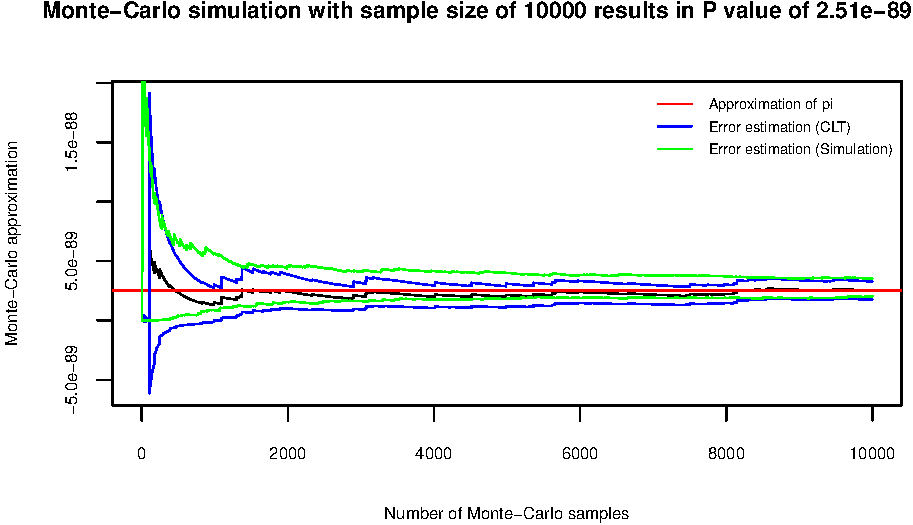
\includegraphics{project1_files/figure-latex/Wahrscheinlichkeit Monte Carlo Transformation-1.pdf}
\caption{Results and error estimation of probability
approximation.\label{fig:plotP}}
\end{figure}

Im Gegensatz zu den obigen naiven Ansätzen ist mittels der
Transformation in gleichverteilte Zufallsvariablen eine Lösung bereits
mit einer relativ kleinen Anzahl von Zufallswerten möglich. Die
Ergebnisse sind in Abbildung \ref{fig:plotP} dargestellt.

\subsection{Approximation eines
Integrals}\label{approximation-eines-integrals}

Die Integrale in den Grenzen zwischen \(0\) und \(1\) zweiter Funktionen
\(h_1(x)\) und \(h_2(x)\) sollen mit Hilfe einer Monte-Carlo
Approximation bestimmt werden.

\begin{equation*}
h_1(x) = (\cos(50x) + \sin(20x))^2 \qquad h_2(x) = \sin(\frac{1}{x})
\end{equation*}

Die Implementierung in \texttt{R} efolgt über zwei Funktionen:

\begin{Shaded}
\begin{Highlighting}[]
\NormalTok{fnIntH1 <-}\StringTok{ }\NormalTok{function(x) \{}
  \CommentTok{# Calculate values of function h1}
  \CommentTok{# }
  \CommentTok{# Args:}
  \CommentTok{#   x: Random values}
  \CommentTok{#   }
  \CommentTok{# Returns:}
  \CommentTok{#   Result of function h1, using random values x as argument}
  \KeywordTok{return}\NormalTok{((}\KeywordTok{cos}\NormalTok{(}\DecValTok{50}\NormalTok{*x)+}\KeywordTok{sin}\NormalTok{(}\DecValTok{20}\NormalTok{*x))^}\DecValTok{2}\NormalTok{)}
\NormalTok{\}}

\NormalTok{fnIntH2 <-}\StringTok{ }\NormalTok{function(x) \{}
  \CommentTok{# Calculate values of function h2}
  \CommentTok{# }
  \CommentTok{# Args:}
  \CommentTok{#   x: Random values}
  \CommentTok{#   }
  \CommentTok{# Returns:}
  \CommentTok{#   Result of function h2, using random values x as argument}
  \KeywordTok{return}\NormalTok{(}\KeywordTok{sin}\NormalTok{(}\DecValTok{1}\NormalTok{/x))}
\NormalTok{\}}
\end{Highlighting}
\end{Shaded}

Wie bei der Bestimmung der Wahrscheinlichkeit oben, kann auch hier
zunächst mit einem naiven Ansatz begonnen werden. Mit Hilfe der
\texttt{integrate}-Funktion von \texttt{R}, soll eine Lösung der
Integrale erfolgen.

\begin{Shaded}
\begin{Highlighting}[]
\CommentTok{# Using R's integrate function to integrate h1}
\NormalTok{h1Int <-}\StringTok{ }\KeywordTok{integrate}\NormalTok{(fnIntH1, }\DecValTok{0}\NormalTok{, }\DecValTok{1}\NormalTok{)}
\NormalTok{h1Int}
\end{Highlighting}
\end{Shaded}

\begin{verbatim}
## 0.9652009 with absolute error < 1.9e-10
\end{verbatim}

Für die Funktion \(h_1(x)\) funktioniert die Bestimmung des Integrals
ohne Probleme. Für die zweite Funktion \(h_2(x)\), kommt es jedoch zu
einem Fehler bei der Berechnung.

\begin{Shaded}
\begin{Highlighting}[]
\CommentTok{# Using R's integrate function to integrate h2}
\KeywordTok{tryCatch}\NormalTok{(\{}
    \KeywordTok{integrate}\NormalTok{(fnIntH2, }\DecValTok{0}\NormalTok{, }\DecValTok{1}\NormalTok{)}
  \NormalTok{\}, }\DataTypeTok{error =} \NormalTok{function(e) \{}
    \KeywordTok{print}\NormalTok{(e)}
  \NormalTok{\})}
\end{Highlighting}
\end{Shaded}

\begin{verbatim}
## <simpleError in integrate(fnIntH2, 0, 1): maximum number of subdivisions reached>
\end{verbatim}

Die Monte-Carlo-Approximation kann beide Integrale annähern. Das
Vorgehen ist weitestgehend anlog zur Bestimmung der Wahrscheinlichkeit
in der vorigen Aufgabe.

\begin{Shaded}
\begin{Highlighting}[]
\NormalTok{fnIntRandom <-}\StringTok{ }\NormalTok{function(n) \{}
  \CommentTok{# Generate random uniform values}
  \CommentTok{# }
  \CommentTok{# Args:}
  \CommentTok{#   n: Size of sample}
  \CommentTok{#   }
  \CommentTok{# Returns:}
  \CommentTok{#   Random vector of size n with values between 0 and 1}
  \KeywordTok{return}\NormalTok{(}\KeywordTok{runif}\NormalTok{(n))}
\NormalTok{\}}
  
\CommentTok{# Set plot panel to two plots}
\KeywordTok{par}\NormalTok{(}\DataTypeTok{mfrow =} \KeywordTok{c}\NormalTok{(}\DecValTok{1}\NormalTok{,}\DecValTok{2}\NormalTok{), }\DataTypeTok{ps =} \DecValTok{9}\NormalTok{, }\DataTypeTok{cex.axis =} \FloatTok{0.9}\NormalTok{, }\DataTypeTok{cex.lab =} \FloatTok{0.9}\NormalTok{)}

\CommentTok{# Using Monte-Carlo integration}
\NormalTok{u <-}\StringTok{ }\KeywordTok{fnIntRandom}\NormalTok{(}\DecValTok{10000}\NormalTok{)}
\NormalTok{h1 <-}\StringTok{ }\KeywordTok{fnIntH1}\NormalTok{(u)}
\NormalTok{h2 <-}\StringTok{ }\KeywordTok{fnIntH2}\NormalTok{(u)}

\CommentTok{# Run error estimation}
\KeywordTok{fnErrorEstimation}\NormalTok{(u, fnIntRandom, }\DataTypeTok{fnValueCalculation =} \NormalTok{fnIntH1)}
\KeywordTok{title}\NormalTok{(}\KeywordTok{paste}\NormalTok{(}\StringTok{"h1: "}\NormalTok{, }\KeywordTok{length}\NormalTok{(u), }\StringTok{" samples, result: "}\NormalTok{,}
            \KeywordTok{round}\NormalTok{(}\KeywordTok{mean}\NormalTok{(h1), }\DecValTok{3}\NormalTok{), }\DataTypeTok{sep =} \StringTok{""}\NormalTok{))}
\KeywordTok{fnErrorEstimation}\NormalTok{(u, fnIntRandom, }\DataTypeTok{fnValueCalculation =} \NormalTok{fnIntH2)}
\KeywordTok{title}\NormalTok{(}\KeywordTok{paste}\NormalTok{(}\StringTok{"h2: "}\NormalTok{, }\KeywordTok{length}\NormalTok{(u), }\StringTok{"samples, result "}\NormalTok{,}
            \KeywordTok{round}\NormalTok{(}\KeywordTok{mean}\NormalTok{(h2), }\DecValTok{3}\NormalTok{), }\DataTypeTok{sep =} \StringTok{""}\NormalTok{))}
\end{Highlighting}
\end{Shaded}

\begin{figure}[htbp]
\centering
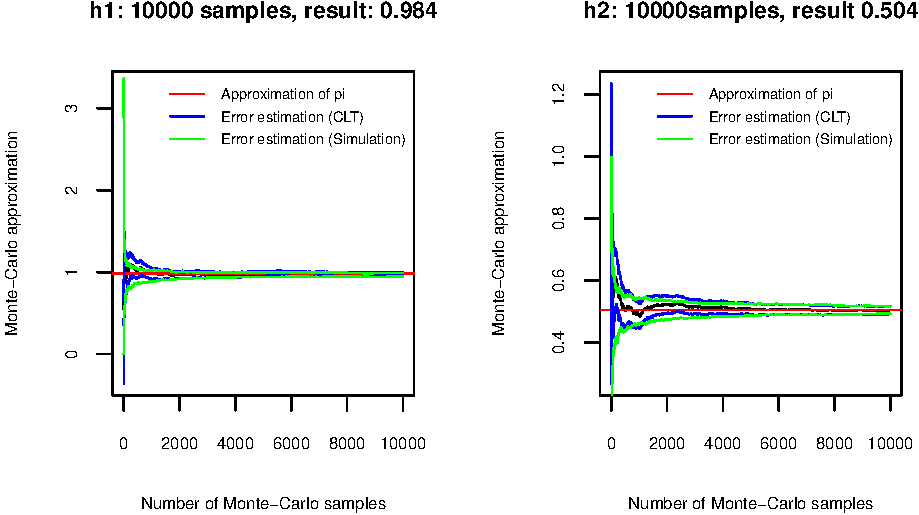
\includegraphics{project1_files/figure-latex/integral monte-carlo-1.pdf}
\caption{Results and error estimation of integral
approximation.\label{fig:plotInt}}
\end{figure}

In Abbildung \ref{fig:plotInt} sind die Ergebnisse und
Fehlerauswertungen der Integral-Approximationen mittels Monte-Carlo
dargestellt. Ein Vergleich der Ergbnisse ist nur für \(h_1(x)\) möglich,
da nur hier die \texttt{integrate}-Funktion von \texttt{R} ein Ergebnis
liefert.

\begin{Shaded}
\begin{Highlighting}[]
\CommentTok{# Calculate percentage error}
\KeywordTok{round}\NormalTok{(}\KeywordTok{abs}\NormalTok{(h1Int$value -}\StringTok{ }\KeywordTok{mean}\NormalTok{(h1))/h1Int$value, }\DecValTok{5}\NormalTok{)}
\end{Highlighting}
\end{Shaded}

\begin{verbatim}
## [1] 0.01924
\end{verbatim}

Es ergibt sich als eine Abweichung von \(\sim 1,924\%\) zwischen der
\texttt{integrate}-Funktion und der Monte-Carlo-Approximation.

\subsection{Erwartungswert der Fläche eines zufälligen
Dreiecks}\label{erwartungswert-der-flache-eines-zufalligen-dreiecks}

Zur einfachen Bestimmung des Erwartungswertes eines zufälligen Dreiecks
kann genutzt werden, dass die Fläche des Dreiecks durch folgende Formel
gegeben ist:

\begin{equation*}
\frac{1}{2}|\text{Det}\,A|,\quad\text{wobei } A = \begin{pmatrix}x_1 & y_1 & 1\\ x_2 & y_2 & 1\\ x_2 & y_2 & 1\\\end{pmatrix}
\end{equation*}

Die Monte-Carlo-Approximation wurde wie folgt implementiert:

\begin{Shaded}
\begin{Highlighting}[]
\NormalTok{fnAreaRandom <-}\StringTok{ }\NormalTok{function(n) \{}
  \CommentTok{# Generate three random uniform values between 0 and 1 for x and y}
  \CommentTok{# respectively. The function directly calculates the area of triangle}
  \CommentTok{# between these three random points.}
  \CommentTok{# }
  \CommentTok{# Args:}
  \CommentTok{#   n: Size of sample}
  \CommentTok{#   }
  \CommentTok{# Returns:}
  \CommentTok{#   Random vector of size n containing area values of random triangles}
  
  \NormalTok{areas <-}\StringTok{ }\OtherTok{NULL}
  \NormalTok{for (i in }\DecValTok{1}\NormalTok{:n) \{}
    \CommentTok{# Generate random values for x- and y-axis}
    \NormalTok{x <-}\StringTok{ }\KeywordTok{runif}\NormalTok{(}\DecValTok{3}\NormalTok{)}
    \NormalTok{y <-}\StringTok{ }\KeywordTok{runif}\NormalTok{(}\DecValTok{3}\NormalTok{)}
    \CommentTok{# Calculate area of trinangle and add to vector}
    \NormalTok{areas[i] <-}\StringTok{ }\KeywordTok{abs}\NormalTok{(}\FloatTok{0.5} \NormalTok{*}\StringTok{ }\KeywordTok{det}\NormalTok{(}\KeywordTok{matrix}\NormalTok{(}\KeywordTok{c}\NormalTok{(x, y, }\KeywordTok{c}\NormalTok{(}\DecValTok{1}\NormalTok{, }\DecValTok{1}\NormalTok{, }\DecValTok{1}\NormalTok{)), }\DataTypeTok{nrow =} \DecValTok{3}\NormalTok{, }\DataTypeTok{ncol =} \DecValTok{3}\NormalTok{)))}
  \NormalTok{\}}
  
  \CommentTok{# Return vector of random triangle areas}
  \KeywordTok{return}\NormalTok{(areas)}
\NormalTok{\}}

\CommentTok{# Set plot panel to one plot}
\KeywordTok{par}\NormalTok{(}\DataTypeTok{mfrow =} \KeywordTok{c}\NormalTok{(}\DecValTok{1}\NormalTok{,}\DecValTok{1}\NormalTok{), }\DataTypeTok{ps =} \DecValTok{9}\NormalTok{, }\DataTypeTok{cex.axis =} \FloatTok{0.9}\NormalTok{, }\DataTypeTok{cex.lab =} \FloatTok{0.9}\NormalTok{)}

\CommentTok{# Generate random triangle area values}
\NormalTok{A <-}\StringTok{ }\KeywordTok{fnAreaRandom}\NormalTok{(}\DecValTok{1000}\NormalTok{)}

\CommentTok{# Run error estimation}
\KeywordTok{fnErrorEstimation}\NormalTok{(A, fnAreaRandom)}
\KeywordTok{title}\NormalTok{(}\KeywordTok{paste}\NormalTok{(}\StringTok{"Monte-Carlo simulation with sample size of "}\NormalTok{, }\KeywordTok{length}\NormalTok{(A),}
            \StringTok{" results in area of "}\NormalTok{, }\KeywordTok{round}\NormalTok{(}\KeywordTok{mean}\NormalTok{(A), }\DecValTok{4}\NormalTok{), }\DataTypeTok{sep =} \StringTok{""}\NormalTok{))}
\end{Highlighting}
\end{Shaded}

\begin{figure}[htbp]
\centering
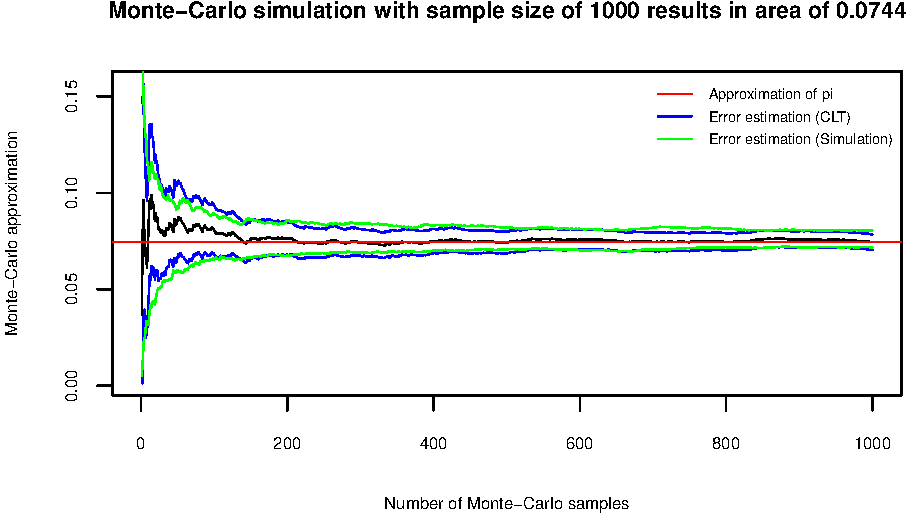
\includegraphics{project1_files/figure-latex/triangle monte-carlo-1.pdf}
\caption{Results and error estimation of random triangle
area.\label{fig:plotTri}}
\end{figure}

Die Ergebniss und die Fehlerauswertung sind in Abbildung
\ref{fig:plotTri} dargestellt.

\newpage

\section{Eine (naive) Datenanalyse}\label{eine-naive-datenanalyse}

Für die naive Datenanalyse am Beispieldatensatz \texttt{faithful} wurden
verschiedene Diagramme erstellt, die eine intuitive Auswertung der Daten
ermöglichen können. Der Datensatz bezieht sich auf erhobene Daten der
Ausstoßzeiten und der Ausstoßdauer des Geysirs ``Old Faithful Geyser''
in den USA.

\subsection{Histogramm}\label{histogramm}

Ein Histogramm stellt die Häufigkeit von Daten dar. Dabei werden Daten
in Klassen (bins) eingeteilt und die jeweilige Häufigkeit von
auftretenden Elementen innerhalb dieser Klasse auf der y-Achse
aufgetragen. Ein Histogramm ermöglicht damit eine erste grobe
Einschätzung der möglichen Verteilung der Daten.

Wird die gesamte Variable \texttt{eruptions} (d.h. Dauer des Ausstoßes)
ausgewertet, ergibt sich ein Histogramm, welches in Abbildung
\ref{histoAll} dargestellt ist. Hierbei wird bereits deutlich, dass es
sich unter Umständen um zwei normalverteilte Teilmengen handelt. Es
könnte also z.B. sein, dass der Ausstoß des Geysirs nach zwei
unterschiedlichen Prozessen abläuft. Ein Blick auf getrennte Daten
(Eruptionszeit größer bzw. kleiner als 3 Minuten), dargestellt in
Abbilung \ref{fig:histoSep}, scheint diese Vermutung zu unterstützen. Ob
es sich jedoch wirklich um normalverteilte Daten handelt kann erst it
dem QQ-Plot (siehe unten) genauer evaluiert werden und ist hier im
besten Fall zu erahnen.

\begin{figure}[htbp]
\centering
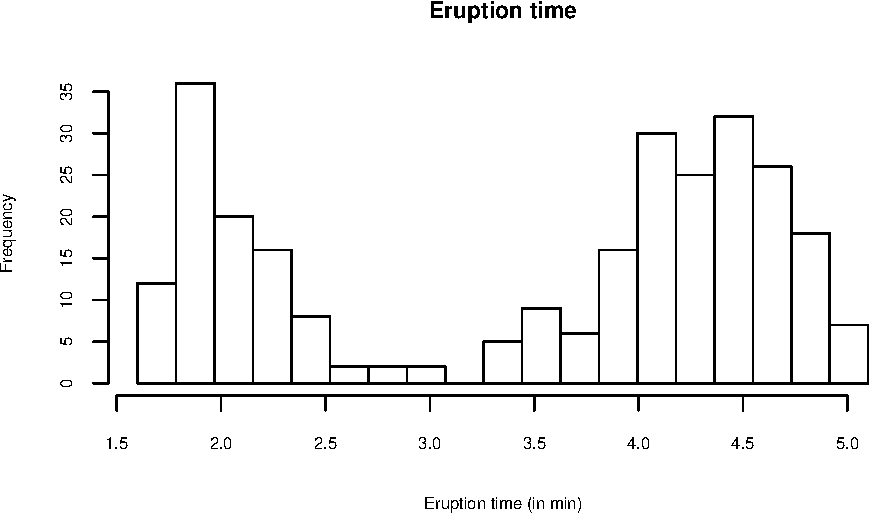
\includegraphics{project1_files/figure-latex/histogram 1-1.pdf}
\caption{Histogram with all eruption data.\label{fig:histoAll}}
\end{figure}

\begin{figure}[htbp]
\centering
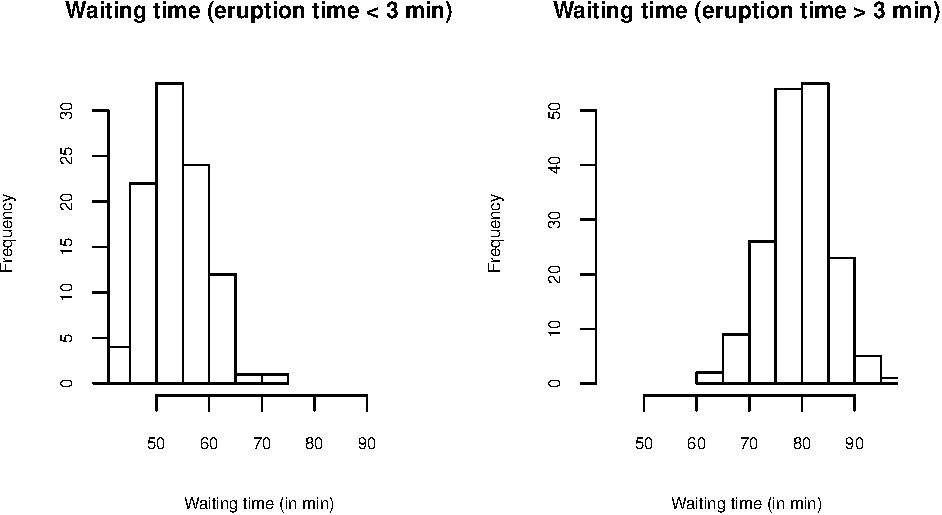
\includegraphics{project1_files/figure-latex/histograms 2-1.pdf}
\caption{Histogram with eruption data, separated in two
categories.\label{fig:histoSep}}
\end{figure}

\subsection{Boxplot}\label{boxplot}

Auch ein Boxplot soll dabei helfen die Verteilung der Daten einschätzen
zu können. Der Boxplot besteht dabei aus drei oder vier Elementen. Es
wird eine Box ausgegeben, deren Kanten den Bereich des unteren und
oberen Quartils abdecken. Innerhalb der Box wird der Median als Linie
eingezeichnet. Zusätzlich werden so genannte Whisker (ebenfalls oben und
unten) eingezeichnet, die sich aus dem \(1,5\)-fachen des
Interquartilsabstands ergeben. Optional können extreme Ausreißer als
Punkte mit dargestellt werden. Der Boxplot gibt damit eine optische
Einschätzung der empirischen Verteilung der Daten.

In Abbildung \ref{fig:box} sind die Wartezeiten für die zwei Untermengen
mit Eruptionszeiten über und unter 3 Minuten dargestellt.

\begin{figure}[htbp]
\centering
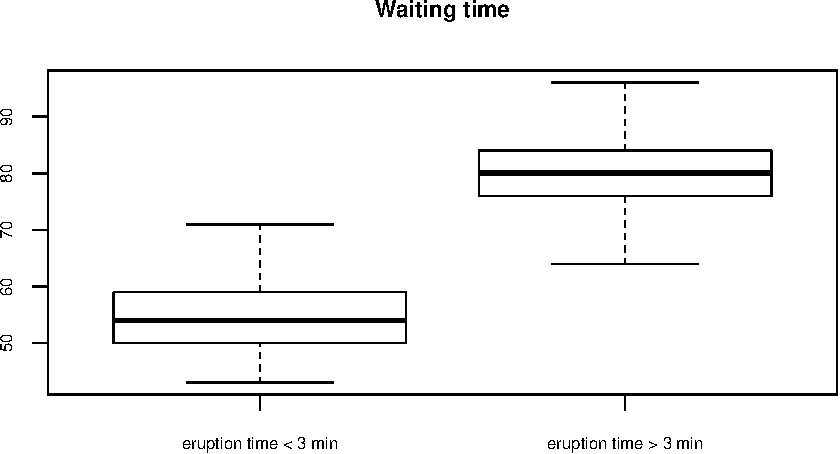
\includegraphics{project1_files/figure-latex/boxplot-1.pdf}
\caption{Boxplot with waiting data, separated in two
categories.\label{fig:box}}
\end{figure}

\subsection{QQ-Plot}\label{qq-plot}

Ein QQ-Plot vergleicht die empirischen Quantile (eine Achse) mit den
theoretischen Quantilen (andere Achse). Wenn die Daten einer
theoretischen Verteilung exakt folgen, liegen alle Punkte somit auf
einer Linie. Mit Hilfe eines QQ-Plots ist es bereits sehr gut möglich
eine Einschätzung darüber zu bekommen, welche konkrete Verteilung den
Daten vermutlich zu Grunde liegt.

In Abbildung \ref{fig:qq} sind alle Varianten dargestellt, d.h.
Eruptions- und Wartzeiten, sowohl für den gesamten Datensatz, als auch
getrennt für solche mit langen Eruptionszeiten (größer 3 Minuten) und
kurzen Eruptionszeiten (kleiner 3 Minuten). Verglichen wird jeweils mit
den theoretischen Quantilen der Standardnormalverteilung. Dabei wird
deutlich, dass die getrennten Daten jeweils vermutlich einzeln
normalverteilt sind, die nicht getrennten Daten ergeben aber kein
solides Bild und sind gemeinsam vermutlich nicht normalverteilt. Dies
spricht sehr dafür, dass die Eruptionen des Gaysirs nach zwei
unterschiedlichen Prozessablaufen.

\begin{figure}[htbp]
\centering
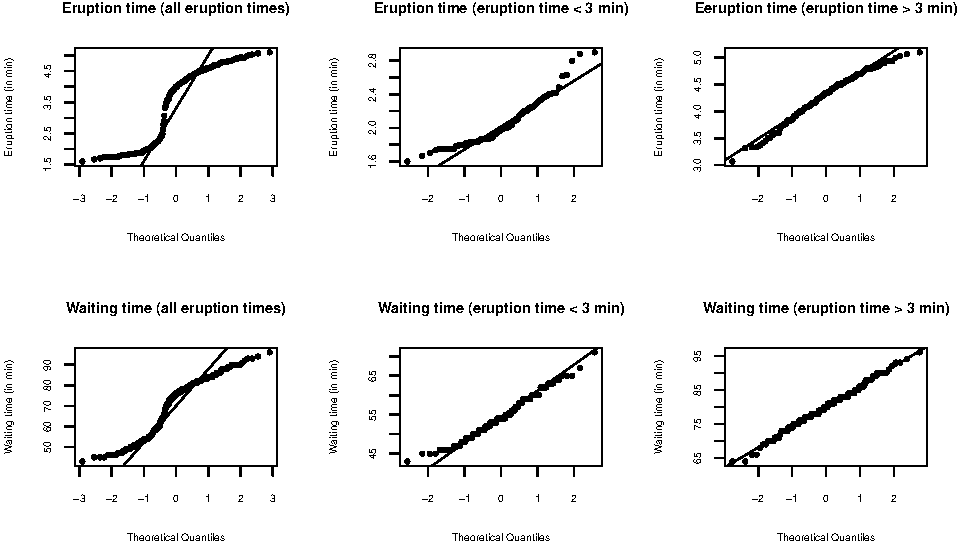
\includegraphics{project1_files/figure-latex/qq-plots-1.pdf}
\caption{QQ-Plots in different data-combination.\label{fig:qq}}
\end{figure}

\subsection{Scatter Plot and
Regression}\label{scatter-plot-and-regression}

Ein Scatter-Plot stellt alle Punkte zweier (oder mehrerer Variablen)
dar. Dabei ist das Ziel Abhängigkeiten zwischen den Variablen
einschätzen können.

In Abbildung \ref{fig:scat} wurden Scatter Plots für alle
Variablen-Kombinationen (analog zu den QQ-Plots) erstellt. Dabei wird
erneut deutlich, dass es zwei Gruppen on Daten gibt. Durch die
Regressionsgeraden wird zusätzlich deutlich, dass es in allen Fällen
signifikante Zusammenhänge (auf einem Niveau von \(\alpha = 5\%\)) gibt.
Die Auswertung der Regressionsanalysen ist hier aus Platzgründen nicht
ausgegeben und ist der Datei \texttt{3.R} zu entnehmen.

\begin{figure}[htbp]
\centering
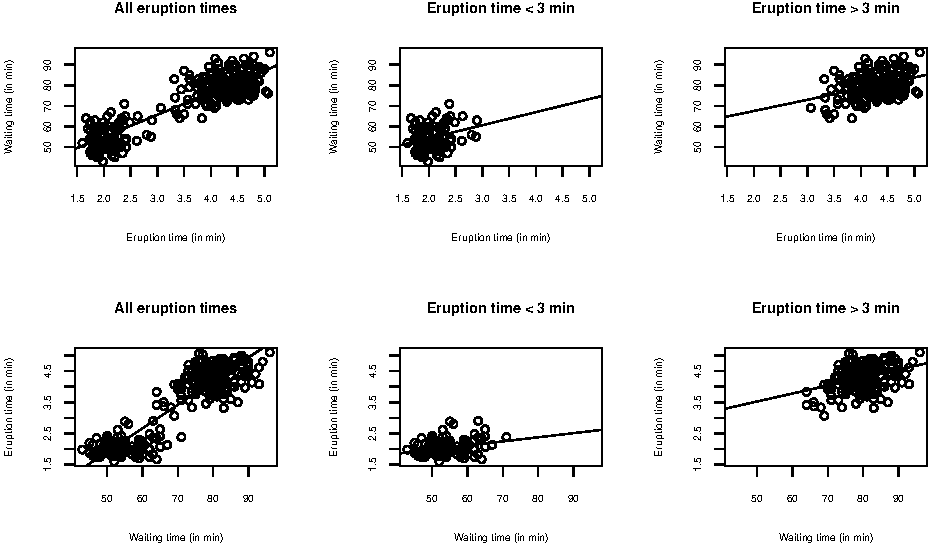
\includegraphics{project1_files/figure-latex/scatter-1.pdf}
\caption{Scatter plots and regression lines in different data
combinations.\label{fig:scat}}
\end{figure}

\subsection{Schätzung}\label{schatzung}

Zuletzt kann eine Schätzung des erwarteten nächsten Ausbruchs erfolgen.
Als Schätzer des Ewartungswerts wird einfachheitshalber der Mittelwert
verwendet, welcher sich im Falle der Normalverteilung aus dem
Maximum-Likelihood-Ansatz und auch aus dem Kleinste-Quadrate-Ansatz
ergibt. Zusätzlich wird der Standard-Fehler bestimmt, also die Varianz
des Schätzers.

Zunächst wird der nächste zu erwartende Ausbruch (Wartezeit) für alle
Daten geschätzt.

\begin{Shaded}
\begin{Highlighting}[]
\CommentTok{# for all eruption times}
\KeywordTok{paste}\NormalTok{(}\StringTok{"mean of waiting time:"}\NormalTok{, }\KeywordTok{round}\NormalTok{(}\KeywordTok{mean}\NormalTok{(faithful$waiting), }\DecValTok{3}\NormalTok{), }\StringTok{"min"}\NormalTok{)}
\end{Highlighting}
\end{Shaded}

\begin{verbatim}
## [1] "mean of waiting time: 70.897 min"
\end{verbatim}

\begin{Shaded}
\begin{Highlighting}[]
\KeywordTok{paste}\NormalTok{(}\StringTok{"standard error of estimator:"}\NormalTok{,}
            \KeywordTok{round}\NormalTok{(}\KeywordTok{sqrt}\NormalTok{(}\KeywordTok{var}\NormalTok{(faithful$waiting)/}\KeywordTok{length}\NormalTok{(faithful$waiting)), }\DecValTok{3}\NormalTok{), }\StringTok{"min"}\NormalTok{)}
\end{Highlighting}
\end{Shaded}

\begin{verbatim}
## [1] "standard error of estimator: 0.824 min"
\end{verbatim}

Im nächsten Schritt wird der nächste erwartete Ausbruch für Ausbrüche
welche weniger als 3 Minuten dauern geschätzt.

\begin{Shaded}
\begin{Highlighting}[]
\CommentTok{# for low eruption times}
\KeywordTok{paste}\NormalTok{(}\StringTok{"mean of waiting time:"}\NormalTok{, }\KeywordTok{round}\NormalTok{(}\KeywordTok{mean}\NormalTok{(faithLow$waiting), }\DecValTok{3}\NormalTok{), }\StringTok{"min"}\NormalTok{)}
\end{Highlighting}
\end{Shaded}

\begin{verbatim}
## [1] "mean of waiting time: 54.495 min"
\end{verbatim}

\begin{Shaded}
\begin{Highlighting}[]
\KeywordTok{paste}\NormalTok{(}\StringTok{"standard error of estimator:"}\NormalTok{,}
            \KeywordTok{round}\NormalTok{(}\KeywordTok{sqrt}\NormalTok{(}\KeywordTok{var}\NormalTok{(faithLow$waiting)/}\KeywordTok{length}\NormalTok{(faithLow$waiting)), }\DecValTok{3}\NormalTok{), }\StringTok{"min"}\NormalTok{)}
\end{Highlighting}
\end{Shaded}

\begin{verbatim}
## [1] "standard error of estimator: 0.593 min"
\end{verbatim}

Zuletzt wird der nächste ewartete Ausbruch für Ausbrüche mit mehr als 3
Minuten Wartezeit geschätzt.

\begin{Shaded}
\begin{Highlighting}[]
\CommentTok{# for high eruption times}
\KeywordTok{paste}\NormalTok{(}\StringTok{"mean of waiting time:"}\NormalTok{, }\KeywordTok{round}\NormalTok{(}\KeywordTok{mean}\NormalTok{(faithHigh$waiting), }\DecValTok{3}\NormalTok{), }\StringTok{"min"}\NormalTok{)}
\end{Highlighting}
\end{Shaded}

\begin{verbatim}
## [1] "mean of waiting time: 79.989 min"
\end{verbatim}

\begin{Shaded}
\begin{Highlighting}[]
\KeywordTok{paste}\NormalTok{(}\StringTok{"standard error of estimator:"}\NormalTok{,}
            \KeywordTok{round}\NormalTok{(}\KeywordTok{sqrt}\NormalTok{(}\KeywordTok{var}\NormalTok{(faithHigh$waiting)/}\KeywordTok{length}\NormalTok{(faithHigh$waiting)), }\DecValTok{3}\NormalTok{), }\StringTok{"min"}\NormalTok{)}
\end{Highlighting}
\end{Shaded}

\begin{verbatim}
## [1] "standard error of estimator: 0.453 min"
\end{verbatim}

Die Schätzer streuen weniger, wenn die Fälle einzeln betrachtet werden
(lange/kurze Ausbrüche). Auch das liefert einen weiteren Hinweis für die
These, dass die Ausbrüche getrennt betrachtet werden sollten.

\newpage

\section{Normalverteilung}\label{normalverteilung}

\end{document}
